\documentclass[10pt]{beamer}
\usetheme{jambro}

\title[]{Microeconomia I - Elementos de Matemática}
\author[]{Paulo Victor da Fonseca}
\date{02 de março de 2023}

\hypersetup{
    colorlinks = true,
    urlcolor = teal,
    linkcolor = white    
}
\usepackage[portuguese]{babel}
\usepackage{subfig}
\usepackage{emoji}

\begin{document}

\begin{frame}[plain]
    \titlepage{
        \begin{center}
            \begin{minipage}{0.8\textwidth}
                \centering
            \end{minipage}
        \end{center}}
\end{frame}

\begin{frame}
    \NB{\emoji{warning} Estas notas de aula servem apenas para sistematizar minha exposi\c{c}\~{a}o, n\~{a}o tendo qualquer
    pretens\~{a}o de originalidade. As proposi\c{c}\~{o}es e demonstra\c{c}\~{o}es que aparecem aqui s\~{a}o retiradas da
    bibliografia citada no programa da disciplina} \bigskip

    \hlight{Leitura sugerida}: Nicholson e Snyder (2019) - Capítulo 2 (seções 2.1 a 2.6)
\end{frame}

\section{Otimização irrestrita univariada}
\begin{frame}
    {Motivação}
    \begin{itemize}
        \item Suponha que uma firma deseje maximizar lucros obtidos com a venda de um determinado bem \bigskip
        \item Suponha, ainda, que os lucros recebidos, $\pi$, dependem apenas da quantidade vendida, $q$, deste bem:\medskip
        \begin{equation}
            \pi = f(q). \label{f_lucro}
        \end{equation}
    \end{itemize}
\end{frame}

\begin{frame}
    {Motivação}
    \begin{center}
		\begin{minipage}[b]{.8\textwidth}
			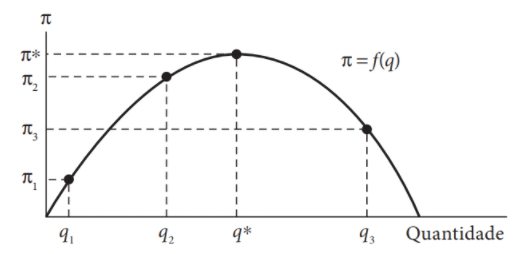
\includegraphics[width=\textwidth]{./figures/aula2_lucro.PNG}\\
			\tiny{{\scshape Função lucro hipotética}. \ Fonte: Nicholson e Snyder (2019).}
            \label{aula2_fig1}
		\end{minipage}
	\end{center}
\end{frame}

\begin{frame}
    {Motivação}
    \begin{itemize}
        \item Pontos $q_1$ e $q_2$ - lucros obtidos variam positivamente com a quantidade produzida:
        \[
            \frac{\Delta \pi}{\Delta q} > 0.
        \] \bigskip
        \item Contanto que $\Delta \pi/\Delta q > 0$, a firma continuará aumentando produção \bigskip
        \item Para pontos à direita de $q^*$, como $q_3$, $\Delta \pi/\Delta q < 0$ e, portanto, o gerente notará que um erro foi cometido \bigskip
        \item Inspeção visual da figura sugere que lucros serão maximizados no ponto $q^*$.
    \end{itemize}
\end{frame}

\begin{frame}
    {Derivadas}
    \begin{itemize}
        \item Um tópico importante em muitas disciplinas científicas, incluindo economia, é o estudo de quão rápido quantidades mudam ao longo do tempo\bigskip
        \item Para calcular a posição futura de um planeta, prever o crescimento populacional de uma espécie biológica, ou estimar a demanda futura de uma determinada \emph{commodity}, precisamos de informações acerca das taxas de variação \bigskip
        \item O conceito usado para descrever a taxa de variação de uma função é o de \hlight{derivada}
    \end{itemize}
\end{frame}

\begin{frame}
    {Derivadas}
    \begin{itemize}
        \item Dada uma função custo total $C = f(Q)$, o custo marginal é definido como a variação no custo total, $C$, resultante de uma pequena variação (infinitesimal) na quantidade produzida, $Q$ \bigskip
        \item O custo marginal pode ser medido pela inclinação da da reta tangente à curva de custo total, que nada mais é que o limite da razão $\Delta C/\Delta Q$ quando $\Delta Q$ tende a zero\bigskip
        \item Assim, o conceito de inclinação da reta tangente a uma curva é a contrapartida geométrica do conceito de derivada
    \end{itemize}
\end{frame}

\begin{frame}
    {Derivadas}
    \NB{Uma fun\c{c}\~{a}o \hlight{$f$ \'{e} diferenci\'{a}vel no ponto $a$} se:
    \[
      \lim_{h \to 0} \frac{f(a + h) - f(a)}{h},  
    \]
    existe. \bigskip

    Neste caso, este limite \'{e} denotado por $f'(a)$ e \'{e} chamado de \hlight{derivada de $f$ no ponto $a$}:
    \[
      f'(a) =   \lim_{h \to 0} \frac{f(a + h) - f(a)}{h}.
    \]\bigskip

    A \hlight{fun\c{c}\~{a}o $f$ \'{e} diferenci\'{a}vel} se $f$ for diferenci\'{a}vel em todos os pontos de seu dom\'{i}nio.
    }
\end{frame}

\begin{frame}
    {Derivadas}
    \begin{itemize}
        \item Na função lucro hipotética que vimos anteriormente, temos:\medskip
        \begin{eqnarray*}
            \left. \frac{d\pi}{d q}\right|_{q = q_1} &>& 0, \\
            \left. \frac{d\pi}{d q}\right|_{q = q_3} &<& 0.
        \end{eqnarray*}
    \end{itemize}
\end{frame}

\begin{frame}
    {Condição de primeira ordem}
    \begin{itemize}
        \item Qual o valor de $d\pi/d q$ avaliada no ponto $q^*$? \bigskip
        \item À esquerda de $q^*$ a derivada da função lucro é positiva, enquanto à direita, é negativa \bigskip
        \item No ponto $q^*$, $f'(q^*) = 0$ \bigskip
        \item Este resultado é geral, \hlight{para uma função contínua e diferenciável $f$ univariada atingir seu valor máximo (mínimo) em um determinado ponto, a derivada da função avaliada neste ponto \textbf{deve} ser igual a zero}: \medskip
        \[
            \left. \frac{d\pi}{d q}\right|_{q = q^*} = \left. \frac{d f}{d q}\right|_{q = q^*} = 0
        \]
    \end{itemize}
\end{frame}

\begin{frame}
    {Condições de segunda ordem}
    \begin{center}
		\begin{minipage}[b]{.8\textwidth}
			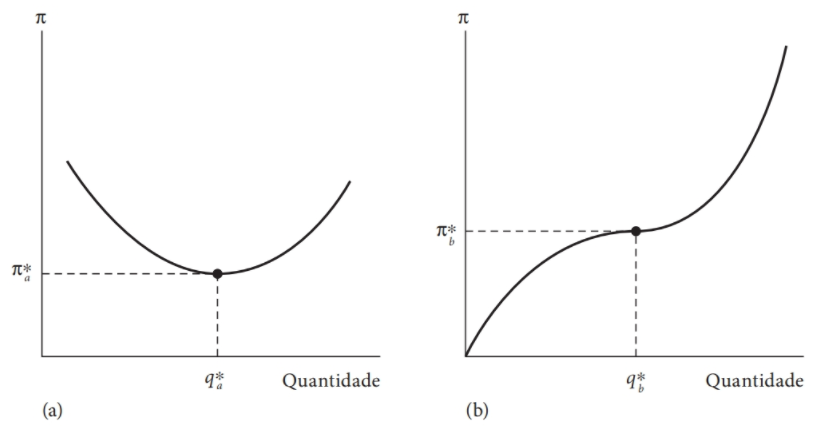
\includegraphics[width=\textwidth]{./figures/aula2_cso.PNG}\\
			\tiny{{\scshape Função lucro - CPOs e CSOs}. \ Fonte: Nicholson e Snyder (2019).}
            \label{aula2_fig2}
		\end{minipage}
	\end{center}
\end{frame}

\begin{frame}
    {Condições de segunda ordem}
    \begin{itemize}
        \item As figuras anteriores evidenciam que $d\pi/d q = 0$ é uma \hlight{condição necessária} mas não \hlight{suficiente} para assegurar um ponto de máximo\bigskip
        \item Para assegurar que o ponto crítico seja, de fato, um máximo (mínimo) relativo, uma segunda condição deve ser imposta\bigskip        
        \item Intuitivamente, os lucros obtidos com a produção de uma quantidade um pouco maior ou um pouco menor que $q^*$ devem ser menores que os lucros associados a $q^*$\bigskip
        \item Matematicamente, se $q < q^*$ devemos ter $d\pi/d q > 0$, e se $q > q^*$ esta derivada deve ser negativa\bigskip
        \item Ou seja, no ponto $q^*$, $d\pi/d q$ deve ser decrescente (negativa)
    \end{itemize}
\end{frame}

\begin{frame}
    {Segundas derivadas e CSOs}
    \begin{itemize}
        \item A derivada de uma derivada é chamada de \hlight{segunda derivada} (ou derivada de segunda ordem) e é denotada por:
        \[
          \frac{d^2 \pi}{d q^2}, \quad f''(q).  
        \]\bigskip
        \item Portanto, a condição adicional para que $q^*$ seja um ponto de máximo local é dada por:
        \[
          \left. \frac{d^2\pi}{d q^2}\right|_{q = q^*} = f''(q^*) < 0.  
        \]
    \end{itemize}
\end{frame}

\begin{frame}
    {Regras de derivação}
    \begin{itemize}
        \item Função constante. $f(x) = c \Rightarrow f'(x) = 0$. \medskip
        \item Dada qualquer constante $a$, $f(x) = x^a \Rightarrow f'(x) = ax^{a-1}$\medskip
        \item Se $f$ e $g$ são funções diferenciáveis, então, $f \pm g$ também é diferenciável e:
        \[
          (f \pm g)'(x) = f'(x) \pm g'(x)  
        \]
        \item Se $f$ e $g$ são diferenciáveis, então, $f \cdot g$ também é diferenciável e:
        \[
          (f\cdot g)'(x) = f'(x)\cdot g(x) + f(x)\cdot g'(x)  
        \]
        \item Se $f$ e $g$ são diferenciáveis em $x$ e $g(x) \neq 0$, então, $f/g$ também é diferenciável em $x$ e:
        \[
          \left(\frac{f}{g}\right)'(x) = \frac{f'(x)\cdot g(x) - f(x)\cdot g'(x)}{g(x)^2} 
        \]
    \end{itemize}
\end{frame}

\begin{frame}
    {Regras de derivação}
    \begin{itemize}
        \item \hlight{Regra da cadeia.} Se $g$ é diferenciável em $x$ e $f$ é diferenciável em $g(x)$, então, $f \circ g$ é diferenciável em $x$ e:
        \[
          (f \circ g)'(x) = f'(g(x))\cdot g'(x)  
        \]
        Alternativamente, se $y = f(x)$ e $x = g(z)$, então:
        \[
          \frac{dy}{dz} = \frac{d y}{d x} \frac{d x}{d z} = \frac{d f}{d x} \frac{d g}{d z}  
        \]
        \item $f(x) = e^x \Rightarrow f'(x) = e^x$ \medskip
        \item $f(x) = a^x \Rightarrow f'(x) = a^x \ln a$ \medskip
        \item $f(x) = \ln x \Rightarrow f'(x) = \frac{1}{x}$
    \end{itemize}
\end{frame}

\begin{frame}
    {Exercícios}
    \begin{enumerate}
        \item Encontre as derivadas das seguintes funções:\medskip
        \begin{enumerate}
            \item $f(x) = (2 - x^2)^3$ \medskip
            \item $f(x) = (x^3 + x^2)^{50}$ \medskip
            \item $f(x) = \sqrt{x^2 + 1}$ \medskip
            \item $f(x) = \frac{3x - 5}{x - 2}$ \bigskip
        \end{enumerate}
        \item Encontre a primeira e segunda derivadas das seguintes funções:\medskip
        \begin{enumerate}
            \item $y = x^3 + e^x$\medskip
            \item $y = \frac{e^x}{x}$\medskip
            \item $y = x^2 \ln x$
        \end{enumerate}
    \end{enumerate}
\end{frame}

\begin{frame}
    {Exercício: maximização de lucros}
    Suponha que a função lucro de uma firma maximizadora de lucros seja dada por:
    \[
      \pi(q) = 1000q - 5q^2.  
    \] \bigskip

    Encontre o valor de $q$ que maximize a função lucro e o valor de lucro máximo.
\end{frame}

\section{Funções multivariadas}
\begin{frame}
    {Funções multivariadas}
    \begin{itemize}
        \item Uma \hlight{função com $n$ variáveis} é uma regra que associa um número $y = f(x_1, \dots, x_n)$ a uma $n$-upla $(x_1, x_2, \dots, x_n)$ de números reais. \bigskip
        \item Exemplo: Em 1928, Charles Cobb e Paul Douglas modelaram o crescimento da economia dos EUA de 1899-1922. Consideraram um modelo no qual a produção é determinada pela quantidade de trabalho utilizada e de capital investido:
        \[
          F(K, L) = A K^\alpha L^{1 - \alpha}  
        \]
        \item A estimativa obtida por MQO foi dada por:
        \[
            F(K, L) = 1,01 K^{0,25} L^{0,75}  
        \]
    \end{itemize}
\end{frame}

\begin{frame}
    {Derivadas parciais}
    \begin{itemize}
        \item Para a função $y = f(x_1, \dots, x_n)$, nosso interesse é o ponto em que $y$ atinge seu valor máximo e nos trade-offs que devem ser feitos para alcançar este ponto\bigskip
        \item Funções de $n$ variáveis: ideia de uma derivada não é bem definida (a inclinação de uma função depende da direção em que é tomada)\bigskip
        \item Usualmente, as inclinações direcionais de interesse são apenas aquelas obtidas quando variamos um dos argumentos mantendo os demais constantes\bigskip
        \item Estas inclinações direcionais são chamadas \hlight{derivadas parciais} e denotamos por:
        \[
          \frac{\partial y}{\partial x_i}, \quad \frac{\partial f}{\partial x_i}, \quad f_{x_i}, \quad f_i  
        \]
    \end{itemize}
\end{frame}

\begin{frame}
    {Derivadas parciais}
    \begin{itemize}
        \item Formalmente, a derivada parcial de $f$ com relação a $x_1$ é:
        \[
          \left.\frac{\partial f}{\partial x_1}\right|_{\bar{x_2},\dots,\bar{x_n}} = \lim_{h\to 0}\frac{f(x_1 + h), \bar{x_2}, \dots, \bar{x_n} - f(x_1, \bar{x_2},\dots,\bar{x}_n)}{h}
        \]
        \item A derivada parcial de uma derivada parcial é chamada \hlight{derivada parcial de segunda ordem}:
        \[
          \frac{\partial (\partial f/\partial x_i)}{\partial x_j} = \frac{\partial^2 f}{\partial x_i\partial x_j} = f_{ij}  
        \]
        \item \hlight{Teorema de Young (Teorema Clairaut-Schwarz)} $f_{ij} = f_{ji}$
    \end{itemize}
    \begin{enumerate}
        \item $f(x_1, x_2) = ax_1^2 + bx_1x_2 + cx_2^2$\medskip
        \item $f(x_1, x_2) = e^{ax_1 + bx_2}$\medskip
        \item $f(x_1, x_2) = a\ln x_1 + b\ln x_2$\medskip
    \end{enumerate}
\end{frame}

\begin{frame}
    {Derivadas parciais}
    \begin{itemize}
        \item Uma derivada parcial de segunda ordem com relação a um mesmo argumento negativa é uma maneira matemática de representar o princípio de rendimentos marginais decrescentes\bigskip
        \item De maneira similar, uma derivada parcial cruzada $f_{ij}$ indica como a efetividade marginal de $x_i$ muda quando $x_j$ aumenta - sinal deste efeito pode ser negativo ou positivo\bigskip
        \item De maneira mais geral, derivadas parciais de segunda ordem contêm informações a respeito da curvatura de uma função\bigskip
        \item A curvatura de uma função é fundamental para determinarmos se um ponto crítico é um ponto de mínimo, máximo (ou nenhum dos casos) em um problema de otimização
    \end{itemize}
\end{frame}

\begin{frame}
    {Regra da cadeia}
    \begin{itemize}
        \item Suponha que $y$ seja uma função cujo domínio seja um subconjunto do $\mathbb{R}^3$: $y = f(x_1, x_2, x_3)$\bigskip
        \item Suponha, ainda, que cada um dos argumentos de $f$ seja função de um único parâmetro $a$, i.e., $y = f(x_1(a),x_2(a),x_3(a))$\bigskip
        \item Temos:
        \[
          \frac{d y}{d a} = \frac{\partial f}{\partial x_1}\frac{d x_1}{d a} +   \frac{\partial f}{\partial x_2}\frac{d x_2}{d a} + \frac{\partial f}{\partial x_3}\frac{d x_3}{d a}
        \]
    \end{itemize}
\end{frame}


\begin{frame}
    {Funções implícitas}
    \begin{itemize}
        \item Se o valor de uma função é mantido constante, cria-se uma relação implícita entre as variáveis independentes\bigskip
        \item I.e., as variáveis independentes não podem assumir valores quaisquer\bigskip
        \item Uma das aplicações desta ideia é a quantificação de trade-offs, inerentes a quase todos os modelos econômicos\bigskip
        \item Aqui, consideraremos o caso mais simples: $\bar{y} = f(x_1, x_2)$
    \end{itemize}
\end{frame}

\begin{frame}
    {Funções implícitas}
    \begin{itemize}
        \item Sob condições relativamente gerais (principalmente $f_2\neq 0$), manter $y$ constante permite a definição de uma \hlight{função implícita} da forma $x_2 = g(x_1)$. Temos, então:
        \[
          \bar{y} = f(x_1, x_2) = f(x_1, g(x_1))  
        \]
        \item Regra da cadeia e diferenciação com relação a $x_1$ implicam:
        \[
            0 = f_1 + f_2 \frac{d g(x_1)}{d x_1}
        \]
        \item Portanto:
        \[
          \frac{d g(x_1)}{d x_1} = \frac{d x_2}{d x_1} = -\frac{f_1}{f_2}  
        \]
    \end{itemize}
\end{frame}

\begin{frame}
    {Funções implícitas: exemplo}
    \begin{itemize}
        \item Considere uma economia descrita por uma fronteira de possibilidades de produção para os bens $x$ e $y$ descrita por:
        \[
          x^2 + 0,25y^2 = 200  
        \]
        \item Se $x = 10$ e $y = 20$, quanto da produção do bem $y$ esta economia deve sacrificar para produzir uma unidade adicional de $x$?
    \end{itemize}
\end{frame}

\section{Otimização irrestrita: funções multivariadas}
\begin{frame}
    {Otimização irrestrita: funções multivariadas}
    \begin{itemize}
        \item O uso de derivadas parciais possibilita a determinação do valor máximo (mínimo) de uma função multivariada\bigskip
        \item Para isso, o uso do conceito de \hlight{diferencial} é importante\bigskip
        \item Para uma função univariada, se $f$ é contínua e diferenciável, denotaremos uma variação arbitrária em $x$ por $d x$\bigskip
        \item Neste caso, a expressão $f'(x) dx$ é chamado o \hlight{diferencial} de $y = f(x)$ e é denotada por $dy$, de modeo que:
        \[
          dy = f'(x)dx  
        \]
        \item Ou seja, $dy$ é proporcional a $dx$, com $f'(x)$ como fator de proporcionalidade
    \end{itemize}
\end{frame}

\begin{frame}
    {Otimização irrestrita: funções multivariadas}
    \begin{itemize}
        \item Como visto anteriormente, a condição necessária para um máximo (mínimo) relativo é dada por $dy = 0$ para pequenas variações em $x$ ao redor do ponto ótimo\bigskip
        \item Portanto, a condição necessária de primeira ordem implica que:
        \[
          f'(x) = 0  
        \]
        \item Estas ideias podem ser aplicadas para o caso de funções multivariadas
    \end{itemize}
\end{frame}

\begin{frame}
    {Otimização irrestrita: funções multivariadas}
    \begin{itemize}
        \item Seja $y = f(x_1,\dots,x_n)$ contínua e diferenciável\bigskip
        \item Poderíamos considerar variar apenas um dos valores das variáveis independentes $x_i$, enquanto mantemos os outros valores constantes\bigskip
        \item O valor do impacto desta variação sobre a variável dependente $y$ seria dado por:
        \[
          dy = f_i dx_i  
        \]
        \item Para que um ponto específico seja um máximo (mínimo) local de $f$, nenhum movimento infinitesimal em qualquer direção pode aumentar o valor desta função\bigskip
        \item Dito de outra forma, todos os termos direcionais similares nesta equação não podem aumentar o valor de $y$
    \end{itemize}
\end{frame}

\begin{frame}
    {Otimização irrestrita: funções multivariadas}
    \begin{itemize}
        \item A única forma para que isso aconteça é que todas as derivadas parciais sejam nulas\bigskip
        \item Formalmente, a condição necessária de primeira ordem para um máximo (mínimo) local é que, neste ponto, tenhamos:
        \[
          f_1 = f_2 = \dots = f_n = 0  
        \]
        \item Um ponto que satisfaça essas condições simultaneamente é chamado \hlight{ponto crítico}\bigskip
        \item Não é, necessariamente, um ponto de máximo (mínimo) relativo a não ser que as condições de segunda ordem sejam satisfeitas\bigskip
        \item Interpretação econômica das CPOs: para que uma função atinja seu valor máximo, é necessário que cada argumento da função cresça até o ponto em que seu valor marginal para a função objetivo seja igual a zero
    \end{itemize}
\end{frame}

\begin{frame}
    {Otimização irrestrita: funções multivariadas}
    Encontre o(s) ponto(s) crítico(s) para a seguinte função de duas variáveis reais:
    \[
      y = f(x_1, x_2) = -(x_1 - 1)^2 - (x_2 - 2)^2 + 10  
    \]
\end{frame}

\section{Otimização com restrições de igualdade}
\begin{frame}
    {Otimização com restrições de igualdade}
    \begin{itemize}
        \item[\emoji{warning}] Até agora: valores máximos de uma função sem restringir escolhas dos argumentos - \hlight{otimização irrestrita}\bigskip
        \item Para a maioria dos problemas econômicos, nem todos os valores que os argumentos de uma função podem assumir são factíveis\bigskip
        \item E.g.: restrição de não-negatividade, restrições por considerações econômicas (restrição orçamentária)\bigskip
        \item Estas restrições podem reduzir o valor máximo da nossa função objetivo. Como não podemos escolher os valores dos argumentos livremente, $y$ pode não ser tão elevado quanto seria no problema irrestrito
    \end{itemize}
\end{frame}

\begin{frame}
    {Otimização com restrições de igualdade}
    \begin{itemize}
        \item Método de solução para problema de otimização com restrições de igualdade: \hlight{método dos multiplicadores de Lagrange}\bigskip
        \item No problema irrestrito, tínhamos um sistema de $n$ equações com $n$ incógnitas ($f_i = 0, \quad \forall i \in 1, \dots n$)\bigskip
        \item No problema restrito temos, pelo menos, uma equação adicional (a restrição), mas nenhuma variável adicional\bigskip
        \item O método dos multiplicadores de Lagrande introduz uma variável adicional (multiplicador de Lagrange) que possibilita a resolução do problema de otimização ($n + 1$ equações simultâneas em $n + 1$ incógnitas)\bigskip
        \item Além disso, veremos durante o curso que esta variável adicional tem uma interpretação econômica útil
    \end{itemize}
\end{frame}

\begin{frame}
    {Otimização com restrições de igualdade}
    \begin{itemize}
        \item Formulação do problema:
        \begin{eqnarray*}
          \max_{x_1, \dots, x_n} & & y = f(x_1, \dots, x_n)  \\
            \text{s.r.} & & g(x_1, \dots, x_n) = c
        \end{eqnarray*}
        onde $g$ representa a relação que deve ser válida entre os valores das variáveis $x$ (restrição) \bigskip
        \item O primeiro passo é definir a \hlight{função Lagrangeana}:
        \[
          \mathcal{L} = f(x_1, \dots, x_n) + \lambda [c - g(x_1, \dots, x_n)],  
        \]
        onde $\lambda$ é a variável adicional - \hlight{multiplicador de Lagrange}
    \end{itemize}
\end{frame}

\begin{frame}
    {Otimização com restrições de igualdade}
    \begin{itemize}
        \item Condições necessárias de primeira ordem:
        \begin{eqnarray*}
            \frac{\partial \mathcal{L}}{\partial x_1} &=& f_1 + \lambda g_1 = 0, \\
            \frac{\partial \mathcal{L}}{\partial x_2} &=& f_2 + \lambda g_2 = 0, \\
            \vdots & \vdots & \ddots \vdots \\
            \frac{\partial \mathcal{L}}{\partial x_n} &=& f_n + \lambda g_n = 0, \\
            \frac{\partial \mathcal{L}}{\partial \lambda} &=& c - g(x_1, \dots, x_n) = 0.
        \end{eqnarray*}
    \end{itemize}
\end{frame}

\begin{frame}
    {Otimização com restrições de igualdade: dualidade}
    \begin{itemize}
        \item Problemas de maximização com restrições possuem um \hlight{problema dual} de minimização condicionada que foca a atenção nas restrições do problema original (primal)\bigskip
        \item Teoria do consumidor: \hlight{problema primal}. Maximização da função utilidade condicionado à restrição orçamentária\bigskip
        \item \hlight{Problema dual}: minimização dos gastos necessários para atingir um nível dado de utilidade
    \end{itemize}
\end{frame}

\begin{frame}
    {Otimização com restrições de igualdade}
    \begin{itemize}
        \item Suponha que um fazendeiro possui uma cerca de comprimento $P$ e deseja cercar a maior área retangular possível\bigskip
        \item Qual o formato de área que este fazendeiro deve escolher?\bigskip
        \item Se o perímetro da área cercada é igual a 400, qual será o comprimento e a largura do terreno cercado?\bigskip
        \item Suponha, agora, que este fazendeiro deseja cercar o terreno de forma a minimizar a quantidade de cerca utilizada para contornar um terreno de área igual a $10.000 m^2$. Qual será o perímetro de área cercada neste caso?
    \end{itemize}
\end{frame}

\begin{frame}{Bibliografia \emoji{books}}
    \begin{itemize}
        \item NICHOLSON, W.; SNYDER C. \emph{Teoria microeconômica: Princípios básicos e aplicações}. Cengage Learning Brasil, 2019. Disponível em: \href{https://app.minhabiblioteca.com.br/books/9788522127030/}{app.minhabiblioteca.com.br/books/9788522127030}
    \end{itemize}
\end{frame}
\end{document}